\chapter{Scripting}

\begin{summary}
This chapter goes deeper into what constitutes a transaction and how scripting is used to lock bitcoins and later unlock them to spend them. Several examples are provided on how to create transactions by calling a node’s API or programmatically.
\end{summary}

\section{Transactions}

A transaction sends bitcoins from one address to another and it consists of 1+ inputs and 1+ outputs. The inputs of a transaction consist of outputs of previous transactions. When an output is spend it can never be used again\footnote{Think of cash. If you give a 20 euro note you can never reuse it. You might be given change but it will be different notes or coins.}. All the bitcoins are transferred elsewhere (to a recipient, back to yourself as change, etc.). Outputs that are available to be spend are called \emph{Unspent Transaction Outputs (UTXOs)} and Bitcoin nodes keep track of the complete UTXO set.

\begin{note}
Each time funds are sent to an address a new output (UTXO) is created. Thus, the balance of an address depends on all the UTXOs that correspond to it. Bitcoin wallets hide UTXOs to make the whole experience friendlier but some wallets allow you to specify which UTXOs you want to spend if needed. When we create transactions programmatically we will deal primarily with UTXOs.
\end{note}

When an output (UTXO) is created we also specify the conditions under which this output can be spend. When you specify an input (the UTXO of a previous transaction) to spend from you have to prove that you satisfy the conditions set by the UTXO.

The spending conditions and the proof that authorizes transfer are not fixed. A scripting language is used to define them. When a new output is created a script is placed in the UTXO called \keyword{scriptPubKey} or more informally locking script.

When we want to spend that UTXO we create a new transaction with an input that references the UTXO that we wish to spend together with an unlocking script or more formally a \keyword{scriptSig}.

The standard transaction output types supported by the Bitcoin protocol are:

\begin{itemize}
\item P2PK (Pay to Public Key - not used anymore)
\item P2PKH (Pay to Public Key Hash)
\item P2SH (Pay to Script Hash)
\item P2WPKH (Pay to Witness Public Key Hash)
\item P2WSH (Pay to Witness Script Hash)
\item OP\_RETURN (allows for storing up to 80 bytes in an output)
\item Multisignature (legacy multisignature transactions; now P2SH/P2WSH is used instead)
\item Non-standard\footnote{Valid Non-standard transactions (containing scripts other than those defined by the standard transaction output type scripts) are rejected and not relayed by nodes. However, they can be mined if it is arranged with a miner.} (any other transaction)
\end{itemize}

The most common transaction output type offering a standard way of transferring bitcoins around is P2PKH (and P2WPKH), which is effectively ``pay to a Bitcoin address''. It is also possible, and used in the past, to pay directly to a public key with P2PK but that is not used anymore. Another very important transaction output type is P2SH (and P2WSH) which allows locking scripts of arbitrary complexity to be used.

To define a locking and unlocking script we make use of a scripting language, simply called \emph{Script}\footnote{https://en.bitcoin.it/wiki/Script}. This relatively simple language consists of several operations each of them identified by an opcode in hexadecimal. It is a simple stack-based language that uses reverse polish notation (e.g. \keyword{2 3 +}) and does not contain potentially dangerous programming constructs, like loops; it is a domain-specific language.

\subsection*{P2PKH}

Let’s examine the standard transaction of spending a Pay to Public Key Hash. The locking script (\keyword{scriptPubKey}) that secures the funds in a P2PKH address is the following:

\begin{emphbox}
\begin{verbatim}
OP_DUP OP_HASH160 <PKHash> OP_EQUALVERIFY OP_CHECKSIG
\end{verbatim}
\end{emphbox}

As we have seen in section \ref{sec:addresses} the public key hash (PKHash) can be derived from the Bitcoin address and vice versa. Thus, the above script locks the funds that have been sent in the address that corresponds to that PKHash.

To spend the funds the owner of the private key that corresponds to that address/PKHash needs to provide an unlocking script that if we prepend to the locking script the whole script will evaluate to true. An unlocking script for a P2PKH will look like this:

\begin{emphbox}
\begin{verbatim}
<Signature> <PublicKey>
\end{verbatim}
\end{emphbox}

% TODO FUTURE SECTION
Using the private key we provide an ECDSA signature of part of the transaction that we create (see future section for more details). We also provide the public key\footnote{As we have already discussed in section~\ref{sec:addresses} the public key only appears in the blockchain after we spend from an address. This is where it appears!} for additional verification.

The validation to spend a UTXO consists of running the script of \keyword{scriptSig} plus \keyword{scriptPubKey}. Both scripts are added in the stack and executed as one script.

\subsection*{Validation of P2PKH Spending}
The validation process is described in below in a step by step explanation during script execution. In each step the script element evaluated will be highlighted (left column) and the current stack (right column) will also be displayed.

%\begin{table}
\begin{center}
\begin{longtable}[H]{ |L{0.47\linewidth}|L{0.47\linewidth}| }
\hline
\multicolumn{2}{|l|}{\emph{Step 0: Execution starts. Stack is empty.}}\\
\hline
\textsf{<Signature> <PublicKey> OP\_DUP OP\_HASH160 <PKHash> OP\_EQUALVERIFY OP\_CHECKSIG} & \\
\hline
\hline
\multicolumn{2}{|l|}{\emph{Step 1: First element is evaluated. It consists of data so it goes into the stack.}} \\
\hline
\textsf{{\color{blue}<Signature>} <PublicKey> OP\_DUP OP\_HASH160 <PKHash> OP\_EQUALVERIFY OP\_CHECKSIG} & \textsf{<Signature>} \\
\hline
\hline
\multicolumn{2}{|l|}{\emph{Step 2: Second element is also data and goes into the stack.}} \\
\hline
\textsf{<Signature> {\color{blue}<PublicKey>} OP\_DUP OP\_HASH160 <PKHash> OP\_EQUALVERIFY OP\_CHECKSIG} & \textsf{<Signature> <PublicKey>} \\
\hline
\hline
\multicolumn{2}{|l|}{\emph{Step 3: Next element is an operator that duplicates the top element of the stack.}}\\
\hline
\textsf{<Signature> <PublicKey> {\color{blue}OP\_DUP} OP\_HASH160 <PKHash> OP\_EQUALVERIFY OP\_CHECKSIG} & \textsf{<Signature> <PublicKey> <PublicKey>} \\
\hline
\hline
\multicolumn{2}{|L{0.94\linewidth}|}{\emph{Step 4: Next element is an operator that calcuates the HASH160 of the top stack element. HASH160 is equivalent to RIPEMD160( SHA256( element ) ) which is what is needed to calculate the PKH from a public key.}}\\
\hline
\textsf{<Signature> <PublicKey> OP\_DUP {\color{blue}OP\_HASH160} <PKHash> OP\_EQUALVERIFY OP\_CHECKSIG} & \textsf{<Signature> <PublicKey> <PKHash>} \\
\hline
\hline
\multicolumn{2}{|L{0.94\linewidth}|}{\emph{Step 5: Next element is data and it is pushed into the stack.}}\\
\hline
\textsf{<Signature> <PublicKey> OP\_DUP OP\_HASH160 {\color{blue}<PKHash>} OP\_EQUALVERIFY OP\_CHECKSIG} & \textsf{<Signature> <PublicKey> <PKHash> <PKHash>} \\
\hline
\hline
\multicolumn{2}{|L{0.94\linewidth}|}{\emph{Step 6: Next element is an operator that checks if the top two elements of the stack are equal and fails the script if they are not. Effectively this validates that the public key provided is indeed the one that corresponds to the PKH (or address) that we are trying to spend.}}\\
\hline
\textsf{<Signature> <PublicKey> OP\_DUP OP\_HASH160 <PKHash> {\color{blue}OP\_EQUALVERIFY} OP\_CHECKSIG} & \textsf{<Signature> <PublicKey>} \\
\hline
\hline
\multicolumn{2}{|L{0.94\linewidth}|}{\emph{Step 7: Next element is an operator that expects two elements from the stack; a signature and a public key that corresponds to that signature. If the signature is valid it returns true, otherwise false.}}\\
\hline
\textsf{<Signature> <PublicKey> OP\_DUP OP\_HASH160 <PKHash> OP\_EQUALVERIFY {\color{blue}OP\_CHECKSIG}} & \textsf{OP\_TRUE} \\
\hline
\end{longtable}
%\caption{Validation steps of P2PKH}
%\label{tab:p2pkh-validation}
\end{center}
%\end{table}

Since the script finished and the only element in the stack is now \keyword{OP\_TRUE}\footnote{Or OP\_1, i.e. true. All the operators, or opcodes, and their explanations can be found at https://en.bitcoin.it/wiki/Script} the node validated ownership of the UTXO and it is allowed to be spent. Success!

To help clarify how addresses, locking scripts and UTXOs relate please see figure~\ref{fig:utxos-pkhashes-addresses}. Addresses 1Zed, 1Alice and 1Bob are short for the actual bitcoin addresses of Zed, Alice and Bob respectively. The diagram emphasises what happens when funds are sent to an address.
\vspace{1em}

\begin{figure}[H]
\begin{center}
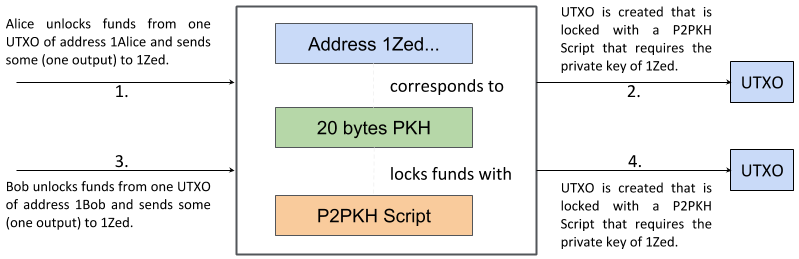
\includegraphics[scale=0.5]{images/utxos-pkhashes-addresses}
\caption{UTXOs, PKHashes and Addresses relationships.}
\label{fig:utxos-pkhashes-addresses}
\end{center}
\end{figure}

This section explained how funds residing in UTXOs are locked/unlocked and how scripts are evaluated for validation. In the next section we will go through several examples of how we can create simple transactions programmatically.



\section{Creating Transactions}

In the previous section we went through transactions, their inputs and outputs and how the funds are locked. In this post we will go through different ways of creating a simple payment transaction from the command line and then programmatically. 

\subsection*{Automatically Create a Transaction}

We can use Bitcoin's build-in command \keyword{sendtoaddress} to send bitcoins to an address.

\begin{emphbox}
\begin{lstlisting}[style=Bash]
$ ./bitcoin-cli sendtoaddress mnB6gSoVfUAPu6MhKkAfgsjPfBWmEEmFr3 0.1
18f23a2c3bea97d30e0e09376222b6888943e7dc86df43ff5dfa1ff59c10d8ec
\end{lstlisting}
\end{emphbox}

In this example we use the node to send \keyword{0.1} bitcoins to a testnet address. Notice that we do not specify any details on which UTXOs to spend from. The node wallet will decide which UTXOs it will spend and in which address the change (there is almost always change) will go; i.e. we do not have any control when sending funds this way.

\begin{note}
Notice that the result is the transaction identifier (txid) of this transaction.
\end{note}


\subsection*{Creating a Transaction using a Node}

In this example we want to select the inputs explicitly. We need to know the txids and the output indexes (vout). As an example, we can get those with:

\begin{emphbox}
\begin{lstlisting}[style=Bash]
$ ./bitcoin-cli listunspent 0
[
  {
    "txid": "b3b7464d3472a9e83da4d5c179620b71724a62eac8bc14ac4543190227183940",
    "vout": 0,
    "address": "n1jnMQCyt9DHR3BYKzdbmXWM8M5UvH9nMW",
    "account": "",
    "scriptPubKey": "76a914ddcf9faf5625d6a96790710bbcef98af9a8719e388ac",
    "amount": 1.30000000,
    "confirmations": 0,
    "spendable": true,
    "solvable": true
  }
  ...
]
\end{lstlisting}
\end{emphbox}

The above command lists all UTXOs (even those with 0 confirmations; i.e. in the mempool). Now we can create a transaction specifying the UTXO that we want to spend.


\begin{emphbox}
\begin{lstlisting}[style=Bash]
$ ./bitcoin-cli createrawtransaction '''
> [
>  {
>   "txid": "b3b7464d3472a9e83da4d5c179620b71724a62eac8bc14ac4543190227183940",
>   "vout": 0
>  }
> ]
> ''' '''
> {
>  "mqazutWCSnuYqEpLBznke2ooGimyCtwCh8": 0.2
> }'''
0100000001403918...efbe09488ac00000000
\end{lstlisting}
\end{emphbox}


The result is the serialized raw transaction in hexadecimal. Note that this is not signed yet. To see the details of the raw transaction we can use:

\begin{emphbox}
\begin{lstlisting}[style=Bash]
$ ./bitcoin-cli decoderawtransaction 0100000001403918...efbe09488ac00000000
{
  "txid": "a7b54334096108e8f69ecfa19263cfbf2f12210165ef5fc2e98ef8e4e466392e",
  "hash": "a7b54334096108e8f69ecfa19263cfbf2f12210165ef5fc2e98ef8e4e466392e",
  "size": 85,
  "vsize": 85,
  "version": 1,
  "locktime": 0,
  "vin": [
   {
    "txid": "b3b7464d3472a9e83da4d5c179620b71724a62eac8bc14ac4543190227183940",
    "vout": 0,
    "scriptSig": {
      "asm": "",
      "hex": ""
    },
    "sequence": 4294967295
   }
  ],
  "vout": [
   {
    "value": 0.20000000,
    "n": 0,
    "scriptPubKey": {
      "asm": "OP_DUP OP_HASH160 6e751b60fcb566418c6b9f68bfa51438aefbe094\\
              OP_EQUALVERIFY OP_CHECKSIG",
      "hex": "76a9146e751b60fcb566418c6b9f68bfa51438aefbe09488ac",
      "reqSigs": 1,
      "type": "pubkeyhash",
      "addresses": [
        "mqazutWCSnuYqEpLBznke2ooGimyCtwCh8"
      ]
    }
   }
  ]
}
\end{lstlisting}
\end{emphbox}

We can confirm that this is unsigned because the unlocking script or \keyword{scriptSig} is empty. We now need to sign this transaction before it becames a valid transaction.

\begin{emphbox}
\begin{lstlisting}[style=Bash]
$ ./bitcoin-cli signrawtransactionwithwallet 01000000014039...be09488ac00000000
{
  "hex": "0100000001403918270...38aefbe09488ac00000000",
  "complete": true
}
\end{lstlisting}
\end{emphbox}

Now we have the final signed raw transaction (in attribute \keyword{hex}). If we use \keyword{decoderawtransaction} now you will see the unlocking script is properly set. We can test if this is a valid transaction before sending it to the node for broadcasting with the \keyword{mempoolaccept} command. Finally, we need to send it to the node for broadcasting.

\begin{emphbox}
\begin{lstlisting}[style=Bash]
$ ./bitcoin-cli sendrawtransaction 0100000001403918270...38aefbe09488ac00000000
error code: -26, error message:, 256: absurdly-high-fee
\end{lstlisting}
\end{emphbox}

In this instance we get an error saying that the transaction has an exceptionally high fee. We have not specified any output for change so \keyword{1.1} bitcoins would be given to miners (\keyword{1.3-0.2}). Most wallets have similar protection mechanisms to help safeguard from user errors.


\subsection*{Using HTTP JSON-RPC}

JSON-RPC is a simple protocol that specifies how to communicate with remote procedure calls using JSON as the format. It can be used with several transport protocols but most typically it is used over HTTP.

A user name and password has to be provided in \keyword{bitcoin.conf}. By default only local connections are allowed, but other connections can be allowed for trusted IPs with the \keyword{rpcallowip} configuration option.

\begin{emphbox}
rpcuser=kostas

rpcpassword=too\_long\_to\_guess
\end{emphbox}

Then we could use a tool like \keyword{curl} to make the JSON-RPC request:

\begin{emphbox}
\begin{lstlisting}[style=Bash]
$ curl --user kostas --data-binary '{"jsonrpc": "1.0", "id":"curltest",  \\
"method": "getblockcount", "params": [] }' -H 'content-type: text/plain;'\\
 http://127.0.0.1:18332/
Enter host password for user 'kostas':

{
  "result": 1746817,
  "error": null,
  "id": "curltest"
}
\end{lstlisting}
\end{emphbox}

Thus, we can also send the commands seen before to construct transactions via JSON-RPC.


\subsection*{Calling Node Commands Programmatically}

A Python library that wraps Bitcoin’s API calls is \keyword{python-bitcoinrpc}. Install with \keyword{pip} and try it out.

\vspace{1em}
\begin{lstlisting}[style=Python]
from bitcoinrpc.authproxy import AuthServiceProxy, JSONRPCException

# user and pw are rpcuser and rpcpassword respectively
user = "kostas"
pw = "too_long_to_guess"     # bad practice - do not hardcode!

rpc_connection = AuthServiceProxy("http://%s:%s@127.0.0.1:18332"%(user, pw))

block_count = rpc_connection.getblockcount()
print(block_count)
\end{lstlisting}
\vspace{1em}

All API calls can be used, including the ones to create a transaction with either \keyword{sendtoaddress} or \keyword{createrawtransaction} + \keyword{signrawtransaction} + \keyword{sendrawtransaction}.



\subsection*{Creating Transactions Programmatically}

The Bitcoin node allows the creation of the basic transactions. It does not support arbitrary scripts. We can create those programmatically by explicitly specifying the locking/unlocking conditions. We will use the \keyword{python-bitcoin-utils} library that can be installed easily with \keyword{pip install bitcoin-utils} in your working python environment.

There are several examples included in the library that you can consult, like the most common transaction, a P2PKH payment\footnote{\url{https://github.com/karask/python-bitcoin-utils/blob/b31c82e7005e06db7f780688cfcd9332d479f39d/examples/p2pkh_transaction.py}} with one input and two outputs (the second output being the change).

\vspace{1em}
\begin{lstlisting}[style=Python]
# Copyright (C) 2018-2020 The python-bitcoin-utils developers
#
# This file is part of python-bitcoin-utils
#
# It is subject to the license terms in the LICENSE file found in the top-level
# directory of this distribution.
#
# No part of python-bitcoin-utils, including this file, may be copied,
# modified, propagated, or distributed except according to the terms contained
# in the LICENSE file.

from bitcoinutils.setup import setup
from bitcoinutils.utils import to_satoshis
from bitcoinutils.transactions import Transaction, TxInput, TxOutput
from bitcoinutils.keys import P2pkhAddress, PrivateKey
from bitcoinutils.script import Script

def main():
    # always remember to setup the network
    setup('testnet')

    # create transaction input from tx id of UTXO (contained 0.4 tBTC)
    txin = TxInput('fb48f4e23bf6ddf606714141ac78c3e921c8c0bebeb7c8abb2c799e9ff96ce6c', 0)

    # create transaction output using P2PKH scriptPubKey (locking script)
    addr = P2pkhAddress('n4bkvTyU1dVdzsrhWBqBw8fEMbHjJvtmJR')
    txout = TxOutput(to_satoshis(0.1), Script(['OP_DUP', 'OP_HASH160', addr.to_hash160(),
                                  'OP_EQUALVERIFY', 'OP_CHECKSIG']) )

    # create another output to get the change - remaining 0.01 is tx fees
    # note that this time we used to_script_pub_key() to create the P2PKH
    # script
    change_addr = P2pkhAddress('mmYNBho9BWQB2dSniP1NJvnPoj5EVWw89w')
    change_txout = TxOutput(to_satoshis(0.29), change_addr.to_script_pub_key())
    #change_txout = TxOutput(to_satoshis(0.29), Script(['OP_DUP', 'OP_HASH160',
    #                                     change_addr.to_hash160(),
    #                                     'OP_EQUALVERIFY', 'OP_CHECKSIG']))

    # create transaction from inputs/outputs -- default locktime is used
    tx = Transaction([txin], [txout, change_txout])

    # print raw transaction
    print("\nRaw unsigned transaction:\n" + tx.serialize())

    # use the private key corresponding to the address that contains the
    # UTXO we are trying to spend to sign the input
    sk = PrivateKey('cRvyLwCPLU88jsyj94L7iJjQX5C2f8koG4G2gevN4BeSGcEvfKe9')

    # note that we pass the scriptPubkey as one of the inputs of sign_input
    # because it is used to replace the scriptSig of the UTXO we are trying to
    # spend when creating the transaction digest
    from_addr = P2pkhAddress('myPAE9HwPeKHh8FjKwBNBaHnemApo3dw6e')
    sig = sk.sign_input( tx, 0, Script(['OP_DUP', 'OP_HASH160',
                                       from_addr.to_hash160(), 'OP_EQUALVERIFY',
                                       'OP_CHECKSIG']) )

    # get public key as hex
    pk = sk.get_public_key().to_hex()

    # set the scriptSig (unlocking script)
    txin.script_sig = Script([sig, pk])
    signed_tx = tx.serialize()

    # print raw signed transaction ready to be broadcasted
    print("\nRaw signed transaction:\n" + signed_tx)


if __name__ == "__main__":
    main()
\end{lstlisting}
\vspace{1em}

This produces the serialized raw transaction in hexadecimal. We can then use \keyword{sendrawtransaction} to send this to the Bitcoin network. Notice that \keyword{bitcoin-utils} wraps the \keyword{python-bitcoinrpc} library in a proxy object so that we can send to a node directly from our python program\footnote{For an example see \url{https://github.com/karask/python-bitcoin-utils/blob/b31c82e7005e06db7f780688cfcd9332d479f39d/examples/node_proxy.py}}.


